\documentclass[a4paper]{article}
\usepackage[utf8]{inputenc}
\usepackage{amsmath}
\usepackage{amsfonts}
\usepackage{amssymb}
\usepackage{url}
\usepackage{graphicx}

\linespread{1.3}

\author{Andrew Rosen}
\title{The Sybil Attack on Peer-to-Peer Networks From the Attacker's Perspective}   % Or The Attacker's View of The Sybil Attack
\begin{document}

\maketitle



%TODO IN THIS ORDER
%1) WRITE PAPER
%2) DO EXPERIMENTS FOR GRAPHS
%3) ADD EXPERIMENT RESULTS TO PAPER
%4) ADD REFERENCES
%5) MAKE UP SOME SLIDES
\begin{abstract}
This paper explores the feasibility of performing naive Sybil attacks on a P2P network that completely occlude healthy nodes from each other.
The vulnerability of Distributed Hash Tables to Sybil attacks and Eclipse attacks has been well known for some time.
However, these vulnerabilities have often been explored in a theoretical sense, assuming the attacker is an all-knowing  and all-powerful global adversary from the beginning.
This paper proves that these are not necessary characteristics and assumptions for an adversary to have to perform a Sybil attack.


We examine the amount of computational effort required to perform an Eclipse attack using only Sybil identities and without poisoning routing tables via false advertisement.
We do this by analyzing the amount of effort it takes for an attacker with a given IP to choose a port to obtain a desired hash key, a process we call \emph{mashing}.
Mashing requires no additional resources on the adversary's end.
Our results showed that an adversary with just 3 IP addresses could compromise 90\% of all connections in a Chord network with 5000 nodes.
While mashing can be used for malicious behavior, we also describe methods and applications for the technique that are beneficial for performing load balancing.
This provides the flexibility for any node to effortless shoulder additional work from bottleneck locations, if acting for the good of the network.
\end{abstract}

\section{Introduction}
One of the key properties of structured peer-to-peer (P2P) systems is the lack of a centralized coordinator.
P2P systems remove the vulnerability of a single point of failure and and the susceptibility to a denial of service attack (cite original Sybil paper), but in doing so, open themselves up to new attacks.
Completely decentralized P2P systems are vulnerable to \textit{Eclipse attacks}, whereby an attacker completely occlude healthy nodes from one another.
This prevents them from communicating without being intercepted by the attacker.

One way to accomplish this attack is to perform a \emph{Sybil Attack} \cite{sybil}.
In a Sybil attack, the attacker creates multiple malicious virtual nodes in order to disrupt the network.
If enough malicious nodes are injected into the system, the majority of the nodes will be occluded from one another, successfully performing an Eclipse attack.

Security analyses typically assumes an adversary using a Sybil is omniscient and can inject virtual nodes wherever he chooses in a reasonable amount of time. 
Our goal is to demonstrate how veracity of that assumption by doing analysis and simulations.

%Why am I doing this?
Sybil attacks represent a significant threat to the security of any distributed system.
Many of the analyses \cite{bauer2007low} on Tor \cite{dingledine2004tor} emphasize the vulnerability of Tor to the Sybil attack.
This threatens the anonymity of Tor users, particularly those living in countries with peculiar notions about personal privacy.

P2P systems like BitTorrent are essential to a wide variety of users.
BitTorrent, for instance, is the \textit{de facto} platform for distributing large files scalably among tens of thousands of clients.
An estimated 20 million peers use BitTorrent daily for sharing and retrieving Linux and BSD-based distros, offline copies of Wikipedia, and personal backup
Current research demonstrates  BitTorrent is vulnerable to the Sybil attack and a persistent attack disabling BitTorrent would e highly detrimental to many users, but especially developers and system administrators\footnote{Perhaps the only reason that BitTorrent hasn't be attacked in such a way as to render it unusable is that those capable of doing so rely heavily upon it.  A sobering thought, since BitTorrent is under an active Sybil attack \cite{sybilbit}. }


There have been many suggestions on how to defend against Sybil attack, but there is no agreed upon ``silver bullet'' among researchers that should be implemented for every distributed application \cite{levine2006survey}
Part of this is surely influenced by the only surefire way to defend against a Sybil attack is to introduce a trusted authority to certify and/or bind identities.
This solution potentially removes the Sybil attack, but reintroduces vulnerabilities to denial of service attacks, bringing us full circle.
Another reason is that there is no single solution for all platforms is that not every solution is compatible with each distributed platform.


Despite the threat represented by the Sybil attack and the research done on the subject, little research has been done from the perspective of an adversary.
We sought to rectify this, both to reemphasize the threat of the Sybil attack, but also because this examination introduces some interesting graph theory problems.

Our work presents the following contributions:
\begin{itemize}
    \item We first discuss the mechanics of performing a Sybil attack and analyze the theoretical effort needed to bring to bear to perform the Sybil attack.
    \item We present our simulations which show how quickly even a naive and inefficient Sybil attack can compromise a system.  We also discuss how a more intelligent attack can be geared to each of the more popular DHT topologies.
    %\item We analyze an interesting graph coloring problem that an attacker needs to solve if the attack is to remain undetected.
    \item We discuss the implications of our work, specifically how the techniques we developed to perform the attack can be used for automatic load balancing.

\end{itemize}

\section{Formal Analysis}




\subsection{Assumptions}
In our analysis we make a few assumptions. 
First, we look primarily at fully distributed systems that assign nodes identifiers using a cryptographic hash function
These are called distributed hash tables (DHTs).
Cryptographic hash functions work by mapping some input value to an $m$-bit key or identifier.
Well-known hash functions for performing this task include MD5 \cite{md5} and SHA1 \cite{sha1}.
Keys generated by the hash function are assumed to be evenly distributed and random \cite{bellare2004hash}. 

In distributed hash tables, $m$ is a large value, in order to avoid collisions between mapped inputs, unintentional or otherwise. 
An $m \geq 128$ is typical, with $m = 160$ being the most popular choice.


Our second assumption is that node IDs are generated by hashing their IP address and port.
The majority of DHTs present this method as the means of generating node IDs, and although other methods exist,\footnote{In Mainline DHT, used by BitTorrent, it appears you can choose your own ID at ``random.''  The horrifying ramifications should be immediately apparent and are discussed in Section \ref{sec:horror}.} they are not nearly as prevalent.

We also assume that nodes store verify that a node's advertised IP address and port generate the advertised node ID. 
Relaxing the latter assumptions would  make the Sybil attack trivial. 
If the attacker does not have to search for values, he can make up any needed key on the fly and falsely advertise it to the network unchallenged.

Consider an attacker operating under these assumptions who wants to inject a malicious node in between two victims.
The attacker must search for a valid IP and port combination under his control that generates a hash key that lies between the two victims's keys, a process we will call \textit{mashing}.
The attackers ability to compromise the network depends on what IP addresses and ports he has available.



\subsection{Analysis}
Suppose we have a DHT with $n$ members in it, with $m$-bit node IDs between $[0,2^{m})$. 
Consider two victim nodes with IDs $a$ and $b$.
The probability $P$ that an attacker can mash a hash key that lands in the range $(a,b)$ is 
$$ P \approx \frac{|b-a|}{2^{m}}\cdot num\_ips \cdot num\_ports  $$

Where $num\_ip$ addresses is the number of IP addresses the attacker has under his control and $num\_ports$ is the number of ports the attacker can try for each IP address.
If the ports the attacker can try are limited the ephemeral ports, the attacker has 16383 ports to use for each IP address.
We can assume that, for a large enough $n$, node IDs will be close to evenly distributed across the keyspace, meaning there will be $\approx \frac{2^{m}}{n}$ keys between each node ID.
This makes the earlier probability equivalent to:
$$ P \approx \frac{1}{n}\cdot num\_ips \cdot num\_ports  $$
This indicates that the ease of mashing is independent to $m$.

The chances of an attacker mashing all $n$ nodes that partition the entire keyspace is:
$$C \approx  1 - (1 -\frac{1}{n})^{num\_ips \cdot num\_ports}  $$


Given a healthy node, the probability $P_{bad\_neighbor}$ that a Sybil is his closest neighbor is:
\begin{equation}
P_{bad\_neighbor} =  \frac{num\_ips \cdot num\_ports}{num\_ips \cdot num\_ports + n - 1}
\label{eq:bad}
\end{equation}
Our experiments in Section \ref{sec:chord} show that $P_{bad\_neighbor}$ is actually the probability that \textit{any} of a nodes links connect to a Sybil.

From the previous equation, the adversary can compute how many unique IP/port combinations they need if they wish to obtain a desired probability $P_{bad\_neighbor}$:

$$ num\_ips \cdot num\_ports =  \frac{n - 1}{1 - P_{bad\_neighbor} }$$

Using our previous assumption that the adversary is limited to the 16383 ephemeral ports, the attacker can computer the number of unique IP addresses needed:
$$ num\_ips  =  \frac{n - 1}{1 - P_{bad\_neighbor} }  \cdot \frac{1}{16383}$$


We verify these equations with our simulations.

\section{Simulations}
An essential part of our analysis was demonstrating just how fast an adversary can compromise a system.
We performed three experiments to accomplish this task.

We used SHA1 for as our cryptographic function, which yields 160-bit hash keys.
Again, we use the constraint that victim nodes do an absolute minimum verification which forces an attacker to only present Sybils with hash keys that he can generate with valid IP and port combinations.

Another important aspect of our simulation is that we do not include the memory resources needed in this analysis.
This is for a couple of reasons, the primary one being that we assume the attacker is capable and competent.
An adversary who wants to use a Sybil attack on a large system would likely roll his own client capable of running on the P2P protocol.
Previous research \cite{mainlinesybil} shows that an adversary peforming a Sybil attack does not need to maintain the state information of other nodes and can leverage the healthy nodes to perform the routing.
Nor does the adversary necessarily create a new running copy for every Sybil created. 

If this was impossible, it is still reasonable to assume the attacker's program would be built to have a minimal memory footprint and drop any messages that require an attacker carry any of the network's load.




%Any application built using a DHT must be address its vulnerabilities to the Eclipse and Sybil attacks

%Security is not something that is thought about for a DHT, unless the 
%DHT is specifically made to be secure against X.  
%Or it's left to the applications





\subsection{Experiment 1: mashing 2 random nodes}
Our initial experiment was designed to establish the feasibility of injecting in between two random nodes.
Each trial, we generated two victims with random IP addresses and ports, and an attacker with a random IP.
The experiment was for the attacker to find a key in between the two victims's key, from the lowest to highest.
The amount of time to mash two random keys was on average 29.6218323708 microseconds, and was achievable $ 99.996\%$ of the time.



%check chord coverage just with the successors
\subsection{Experiment 2:  Nearest Neighbor Eclipse via Sybil}
The objective of the second experiment is to completely ensnare a network using a Sybil attack, starting with a single malicious node.
With simulate this by creating a network of $n$ nodes.  
Each node is represented by a key generated by taking the SHA1 of a random IP/port combination.
The goal of the attacker is to insert a Sybil in between as many of the nodes as possible.
We call this the \textit{Nearest Neighbor Eclipse} since the attacker seeks to block as many lines of communication between neighboring nodes as possible.

The attacker is given a randomly generated $num\_ips$ IP addresses, but can use any port between 49152 and 65535.
This gives the attacker $ 16383 \cdot num\_ips $ possible hash keys to use for Sybils.
The attacker can easily precompute all of theses hash keys and store them in a sorted list to be used as needed.
This requires only $160  \cdot 16383 = 2621280$  bits, or about 320 kilobytes for each set of hash keys generated for an IP.\footnote{We can ignore the cost of having to store 32 bits for each IPv4 address and 16 bits required by each port with some clever mapping and indexing.}

To perform the attack, an adversary choses any random hash key as a starting point to ``join'' the network.
This is his first Sybil and the join process provides information about a number of other nodes.
Most importantly,  nodes provide information about other nodes that are close in the hash space, which provided to enable fault tolerance between immediate neighbors.
The adversary uses this information to inject Sybils in between successive healthy nodes.


For clarity we present this example. 
Consider the small segment of the network made up of adjacent nodes $a$, $b$, $c$, and $d$.
The Sybil joins between nodes $a$ and $b$, and the joining process informs the adversary about node $c$, possibly node $d$, and a handful of other nodes in the network.
The adversary will always learn about node $c$ because a normal node between $a$ and $b$ would need to know about node $c$ for fault tolerance.

The adversary's next move would be to inject a node between nodes $b$ and $c$.
This is done by selecting a precomputed hash key $k$, such that $b \leq k \leq c$.
The adversary injects a Sybil node with key $k$, which joins in between $b$ and $c$, and the joining process informs the adversary about node $d$ and several other nodes, including many close nodes.
The adversary then aims to inject a node in between $c$ and $d$, and continues \textit{ad nauseam}.

Depending on the network size and the number of keys available to the adversary, it is entirely possible the adversary will not have a key to inject between a pair of successive nodes.
In this case, the node moves on to the successive pair that the node has learned about.


We simulated this attack on networks of up to size 20,000,000.
We gave the attacker access to up to 19 IP addresses.
We presents our results in Figures \ref{fig:exp2} and \ref{fig:size_prob_all} and Table \ref{tab:exp2}.
For Table \ref{tab:exp2}, we have included only the results for larger sized networks, as the smaller sized networks were completely dominated.


\begin{figure}
\centering
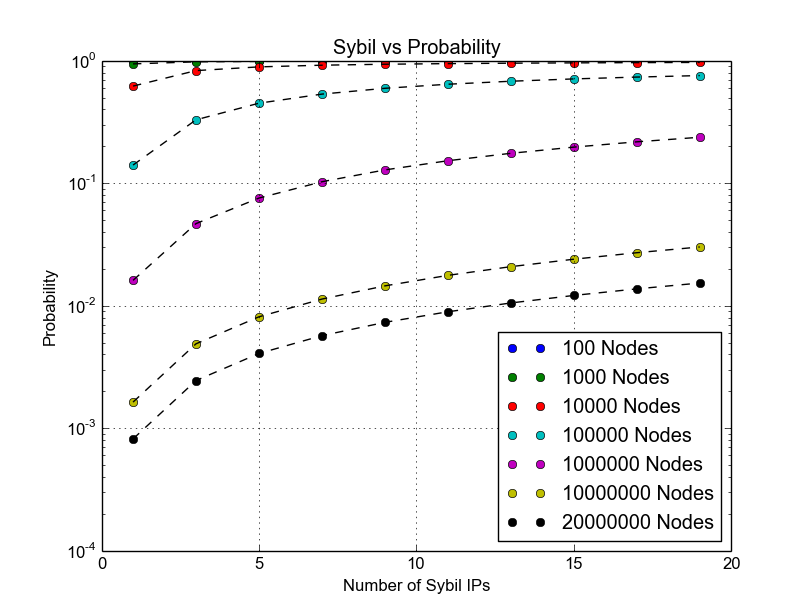
\includegraphics[width=1\linewidth]{ip_prob_all}
\caption[foo]{Our simulation results.  
    The $x$-axis corresponds to the number of IP addresses the adversary can bring to bear.
    The $y$-axis is the probability that a random region between two adjacent normal members of the network can be mashed.
    Each line maps to a different network size of $n$.
    The dotted line traces the line corresponding to the Equation \ref{eq:bad}: $ P_{bad\_neighbor} =  \frac{num\_ips \cdot 16383}{num\_ips \cdot 16383 + n - 1}$}.
\label{fig:exp2}
\end{figure}


\begin{figure}
\centering
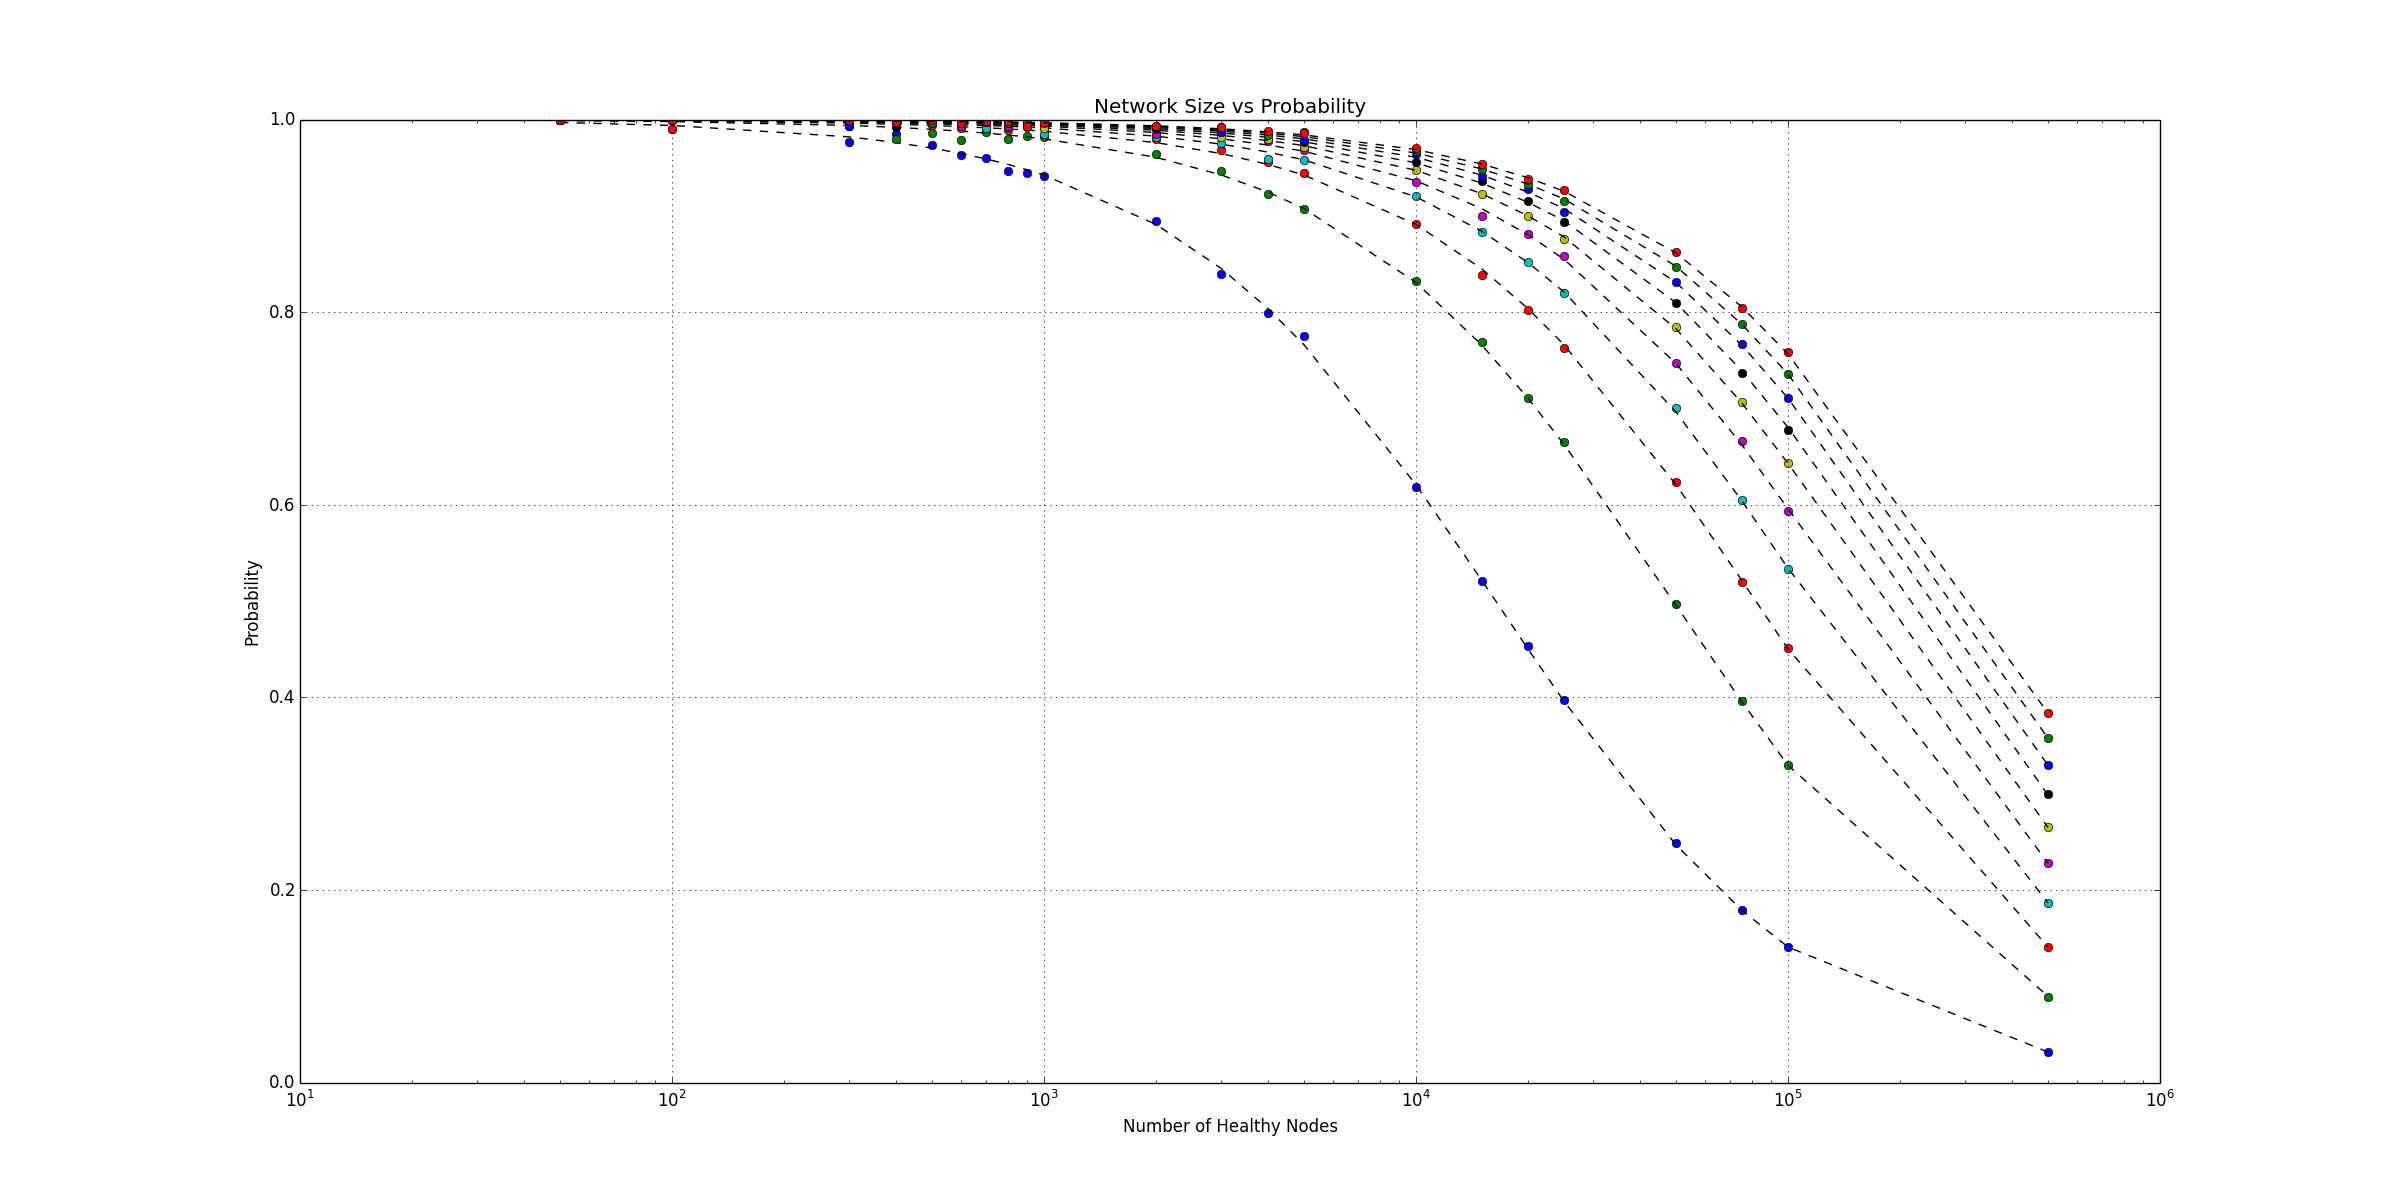
\includegraphics[width=\linewidth]{size_prob_all}
\caption[a]{These are the same as results shown in Figure \ref{fig:exp2}, but our $x$-axis is the network size $n$ in this case.  
    Here, each line corresponds to a different number of unique IP addresses the adversary has at their disposal.}
\label{fig:size_prob_all}
\end{figure}



\begin{table}[h]\small

\begin{center}
       
\begin{tabular}{|r|r|r|r|}
    \hline
    Sybil IPs & Network Size & \% of Regions Injected & Sybils/Region \\ \hline
1.0 & 5000.0 & 0.7748 & 3.2762 \\ \hline
1.0 & 5000000.0 & 0.0032654 & 0.0032768 \\ \hline
1.0 & 10000000.0 & 0.0016364 & 0.0016384 \\ \hline
1.0 & 20000000.0 & 0.00081865 & 0.0008192 \\ \hline
5.0 & 5000.0 & 0.9444 & 16.381 \\ \hline
5.0 & 5000000.0 & 0.0161208 & 0.016384 \\ \hline
5.0 & 10000000.0 & 0.0081223 & 0.008192 \\ \hline
5.0 & 20000000.0 & 0.0040801 & 0.004096 \\ \hline
11.0 & 5000.0 & 0.9708 & 36.0428 \\ \hline
11.0 & 5000000.0 & 0.0347646 & 0.0360448 \\ \hline
11.0 & 10000000.0 & 0.0177117 & 0.0180224 \\ \hline
11.0 & 20000000.0 & 0.008932 & 0.0090112 \\ \hline
19.0 & 5000.0 & 0.9834 & 62.2452 \\ \hline
19.0 & 5000000.0 & 0.058562 & 0.0622592 \\ \hline
19.0 & 10000000.0 & 0.0301911 & 0.0311296 \\ \hline
19.0 & 20000000.0 & 0.01532465 & 0.0155648 \\ \hline
\end{tabular}
\label{tab:exp2}
\caption{Results for Sybil Attack.  The Fraction of regions injected is the percentage of all regions for which the adversary could inject a Sybil with the suitable key. The Sybil/Region measure is how many Sybils were available to inject a particular region on average.}
\end{center}

\end{table}

%NEED TO TEST TO SEE WHAT NEEDED TO ATTACK 50,000,000 size network, twice the size of the BitTorrent network.  CAN WE?
%Each experiment took less than a second to perform.
Our results show that an adversary, given only modest resources, can inject a Sybil in between the vast majority of successive nodes in moderately sized networks.
In a large network, modest resources still can be used to compromise more that a third of the network, an  important goal if the adversary  wishes to launch a Byzantine attack.

Our results match values predicted by \ref{eq:bad}.
However, this experiment only covers the short links of the network, but not the long distance links.



\subsection{Experiment 3: Fully Complete Eclipse via Sybil}
\label{sec:chord}
We extended the previous experiment by considering the long-distance hops of each node in addition to the short-range links of the DHT.
We choose to model an attack on a P2P system built using Chord \cite{chord}.
We did this for a number of reasons.
Chord is an extremely well understood DHT and is very simple to evaluate using simulations.
Nodes in Chord generate long distance links independent of information provided by other nodes, rather than directly querying neighbors.
This prevents adversaries from poisoning the node's routing table via false advertisements, which can be on other DHTs such as Pastry \cite{pastry}. 
A Sybil attack the most straightforward means of effecting an Eclipse attack on a Chord network.

Nodes in Chord have $m$ long-range links, one for each of the bits in the keys, which is 160 in our experiments.
Each of node $a$'s long-range hops points to the node with the lowest key $\geq a + 2^{i} \mod 2^{m} , 0 \leq i \leq 160$.


The attack is very similar to the Nearest Neighbor attack demonstrated above.
Beside injecting a node in between successive nodes, the attacker also attempts to place a Sybil in between each of the long-range links.
We simulated this attack under the same parameters as above and are presented in Table \ref{tab:exp3}.




\begin{table}[h]\small
    
    \begin{center}
        
        \begin{tabular}{|r|r|r|r|}
            \hline 
            IPs & Network Size &  \% links occluded & Occlusion per node \\ \hline
            1 & 1000 & 0.94186875 & 150.699 \\ \hline
            1 & 10000 & 0.618480625 & 98.9569 \\ \hline
            1 & 100000 & 0.141753625 & 22.68058 \\ \hline
            3 & 1000 & 0.97915625 & 156.665 \\ \hline
            3 & 10000 & 0.83425 & 133.48 \\ \hline
            3 & 100000 & 0.3286290625 & 52.58065 \\ \hline
            5 & 1000 & 0.988725 & 158.196 \\ \hline
            5 & 10000 & 0.894415 & 143.1064 \\ \hline
            5 & 100000 & 0.4488916875 & 71.82267 \\ \hline
            7 & 1000 & 0.99091875 & 158.547 \\ \hline
            7 & 10000 & 0.919071875 & 147.0515 \\ \hline
            7 & 100000 & 0.5337635625 & 85.40217 \\ \hline
            9 & 1000 & 0.9948125 & 159.17 \\ \hline
            9 & 10000 & 0.935495625 & 149.6793 \\ \hline
            9 & 100000 & 0.5936118125 & 94.97789 \\ \hline
            
            
        \end{tabular}
        \label{tab:exp3}
        \caption{Results for Sybil Attack on Chord. The percentage of links occluded is the percentage of long range links from healthy nodes that connect to Sybil nodes. 
            The Occlusion per node measures how many of the 160 long range links lead to a Sybil on average.  
            We ignore the predecessor links since it is not used for routing.}
    \end{center}
    
    
    
\end{table}

\begin{figure}
    \centering
    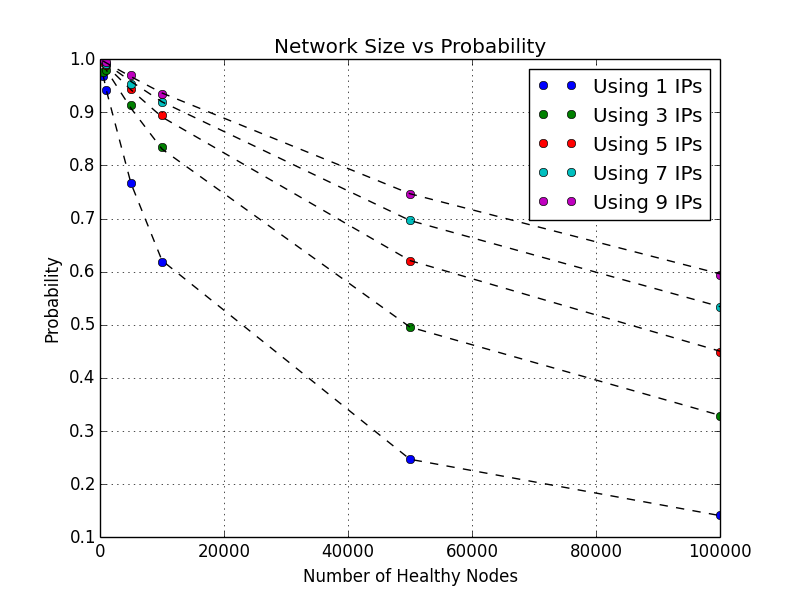
\includegraphics[width=\linewidth]{size_occlusion_chord}
    \caption{This graph shows the relationship between the network size and the probability a particular link, adjacent or not, can be mashed.
        The dotted line traces the line corresponding to the Equation \ref{eq:bad}: $ P_{bad\_neighbor} =  \frac{num\_ips \cdot 16383}{num\_ips \cdot 16383 + n - 1}$.}
    
    \label{fig:exp3}
\end{figure}



Surprisingly, the percentage of links from healthy nodes that connect to Sybil nodes follows \ref{sec:chord}.
We can calculate that the number of IP addresses needed to compromise half the links in a 20,000,000 node Chord network is 2442.



%\subsubsection{Plaxton Based networks}


%\section{Masking the Attack}
%Now that we have established that a Sybil attack can be performed with great ease, our focus now turns to avoiding detection.
%The only surefire way to achieve this is by preventing a node from seeing 
%We need a different IP for each point surrounding our victim.  In the Nearest-Neighbor attack, we need a 

%We can reduce this into an interesting graph coloring problem.


%The hard maximum, in general, is $m$ separate IP addresses, one for each bit in a $\log n$ routing/routing table DHT.
%Recall that the vast

\section{Conclusions and Future Work}
%\section{Simple Load Balancing Injection Framework}
\label{sec:horror}

Our analysis and experiments show that an adversary with a small number of machines and limiting their port usage to just the ephemeral ports can easily compromise a P2P system and mash the majority of the regions between nodes.
This effectively prevents nodes from talking to one another without first sending messages through Sybils, who can eavesdrop on them or disregard the eaves and move straight on to the dropping.

Our discussion have primarily concerned Chord, but an astute reader may wonder why did we not simulate an attack on Mainline DHT (MLDHT) \cite{mainline}, the Kademlia \cite{kademlia} based DHT used as the backend of BitTorrent.
It is ostensibly the largest P2P system in use, so it seems more suited for analyzing our mash-based attack than Chord.

We avoided simulating the mashing process on MLDHT because it is completely unnecessary to perform the attack.
In MLDHT, a node ID is not chosen by hashing an IP and port combination, but by picking an address uniformly at random between 0 and $2^{160}-1$.
An adversary who wants to a completely isolate a node on the network can choose Sybils with ``random'' hashkeys completely eliminate that node from the routing tables of healthy peers. 
Research has examined Mainline's vulnerability to Sybil attacks\cite{sybilbit} and detected entities performing the attack on Mainline.
Our research demonstrates that switching to using a SHA1 hash of the IP and port is no defense against a Sybil attack, since the adversary can easily mash into appropriate places.
%A big difference is their honeypots target those who respond to everything.

However, the mashing process can be used in non-security related settings to benefit a DHT.
As we have mention previously, the SHA1 hash has an evenly distributed output, but no set of keys will be completely evenly distributed.
Some nodes will be responsible for larger regions than others\footnote{More susceptible to a mash.} and be responsible for a larger portion for the work.

If a node can detect a when a peer has too much of a load, the node can inject a virtual node into the region to shoulder some of the load.
Too much of a load could be defined by having a too large region or by watching traffic requests.
This could be integrated into a distributed key allocation system, so that a node can bind these keys to itself, but only use a small portion of the keys alloted to it to aid with load-balancing.
The only cost would be that node would have to keep track of the keys it can inject, which we mentioned was only 320 kilobytes of data.


\bibliography{potato}
\bibliographystyle{plain}
\end{document}
